\documentclass{article}

\usepackage{amsmath}
\usepackage{listings}
\usepackage{color}
\usepackage{placeins}
\usepackage{graphicx}
\graphicspath{ {C:\Users\Dell\Documents\Graduate - Economics\Empirical Industrial Organisation I\pset1_working} }

\title{Empirical Industrial Organisations I: PSet 1}
\author{S M Sajid Al Sanai}
\date{November 2, 2018}

\begin{document}

\maketitle
\pagenumbering{arabic}
\tableofcontents

\lstset{
	frame=lines,
	basicstyle=\small\sffamily,
	tabsize=4,
	columns=fixed,
	showstringspaces=false,
	showtabs=false,
	keepspaces,
	commentstyle=\color{red},
	keywordstyle=\color{blue}
}

\newpage
\section{Section I}
\subsection{Question 1}

\subsubsection{(a) Case for 3 Products across 100 Markets}
Using the simulated data for the 3 product and 100 markets case calculated at the true parameters $\theta=\{\alpha, \beta, \sigma_\alpha\}$ and $\gamma$, I obtained the distributions for Prices, Profits, and the Consumer Surplus detailed below. Graphs for products 1-3 are aligned side-by-side for comparison.
\par Distribution of prices for product 1 exhibit some bimodality and is centred around USD 3 - USD 4. Distribution of prices for product 2 appears skewed slightly toward lower prices and seems centred around USD 2. Distribution of prices for product 3 appears more normally distributed around average prices of USD 3. Profits are distributed relatively similarly across products with products 2 and 3 earning some higher profits than product 1. Consumer Surplus exhibits somewhat of a bimodal distribution, with a centred mean.

\begin{figure}[h]
  \caption{Distribution of Prices}
  \centering
    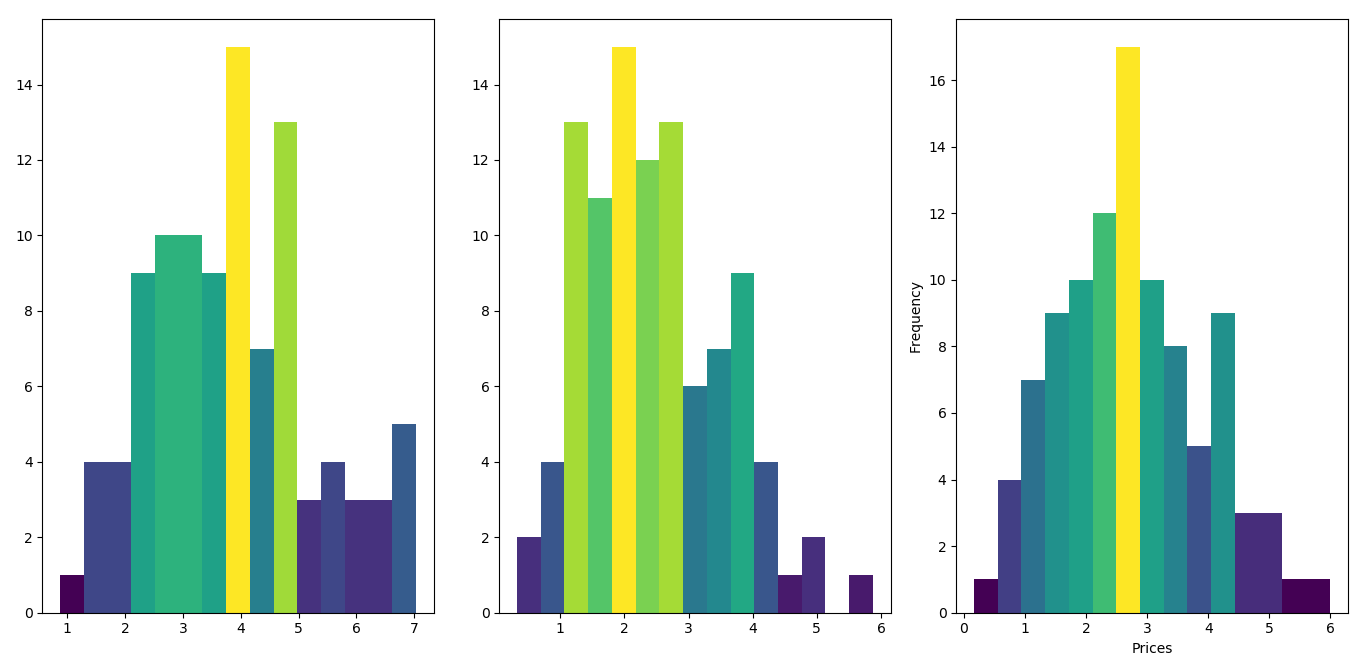
\includegraphics[width=1.0\textwidth]{fig_hist_prices3_t}
  \caption{Distribution of Profits}
  \centering
    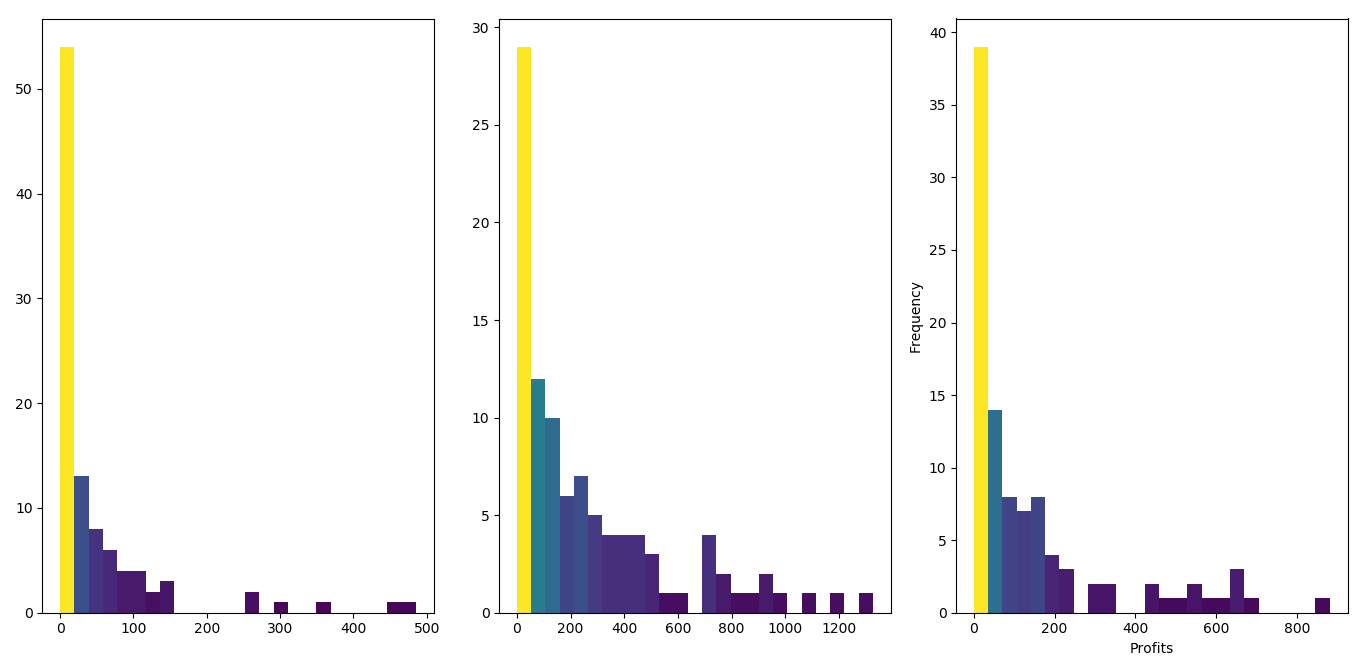
\includegraphics[width=1.0\textwidth]{fig_hist_profits3_t}
  \caption{Distribution of Consumer Surplus}
  \centering
    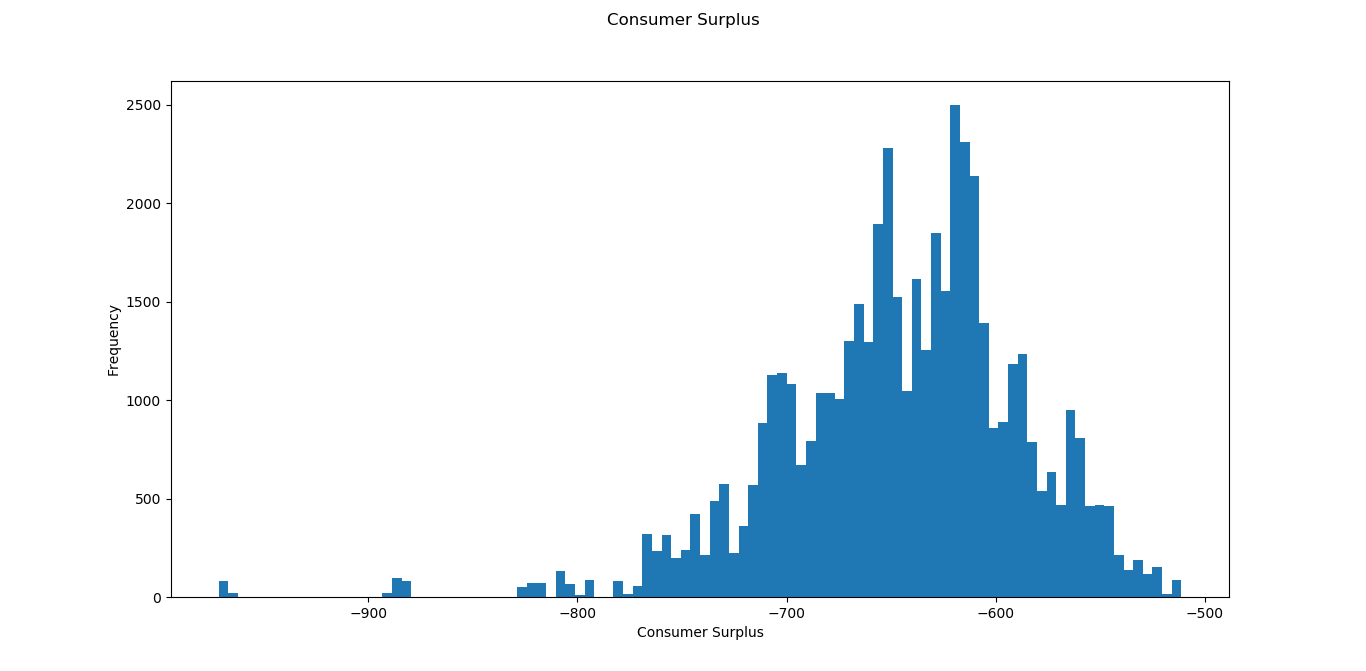
\includegraphics[width=1.0\textwidth]{fig_hist_consumersurplus3_t}
\end{figure}
\FloatBarrier

\subsubsection{(b) Case for 5 Products across 100 Markets}
Using the simulated data for the 5 product and 100 markets case calculated at the true parameters $\theta=\{\alpha, \beta, \sigma_\alpha\}$ and $\gamma$, I obtained the distributions for Prices, Profits, and the Consumer Surplus detailed below. Graphs for products 1-5 are aligned side-by-side for comparison.
\par Distribution of prices for products 1, 3, and 5 exhibit normal distribution with centring at an average price in each instance. Product 2 exhibits some bimodality. Distribution of prices for product 4 are largely skewed to negligible low average prices. Profits are distributed relatively similarly across products 1-3, and 4-5. Products 4 and 5 earning considerably higher profits than products 1-3. Consumer Surplus exhibits a normal distribution with flat tails and a centred mean.

\begin{figure}[h]
  \caption{Distribution of Prices}
  \centering
    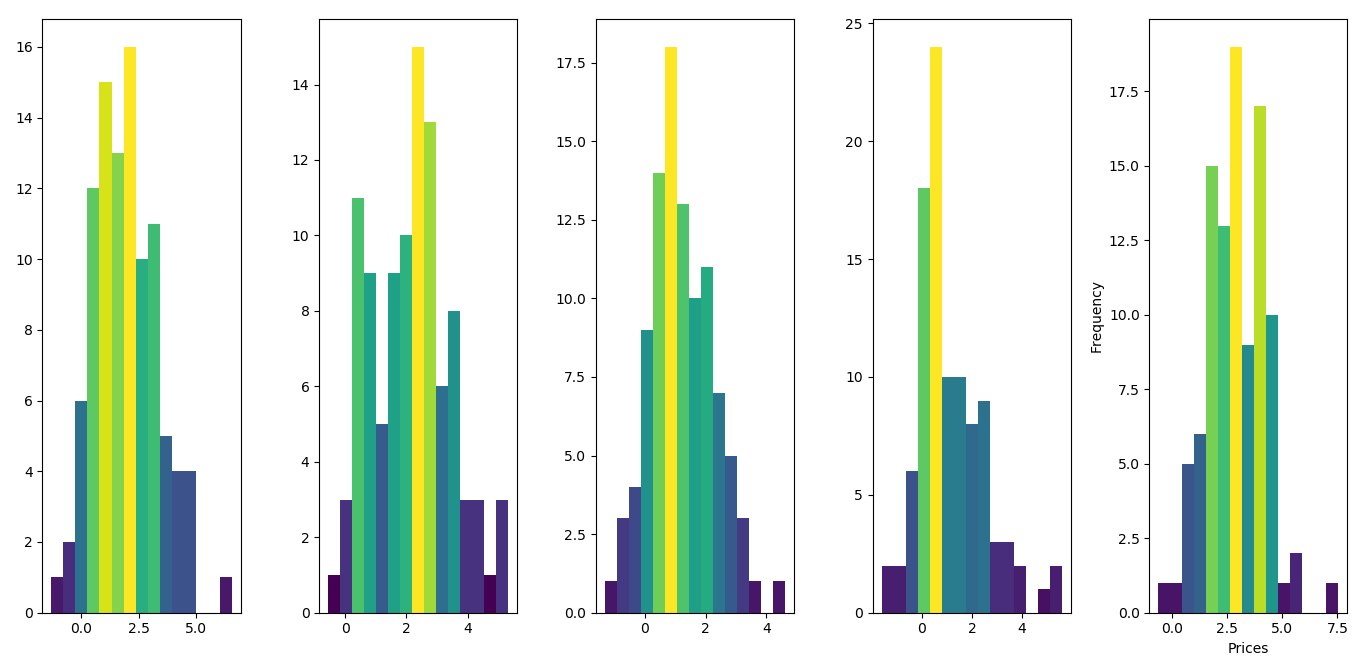
\includegraphics[width=1.0\textwidth]{fig_hist_prices5_t}
  \caption{Distribution of Profits}
  \centering
    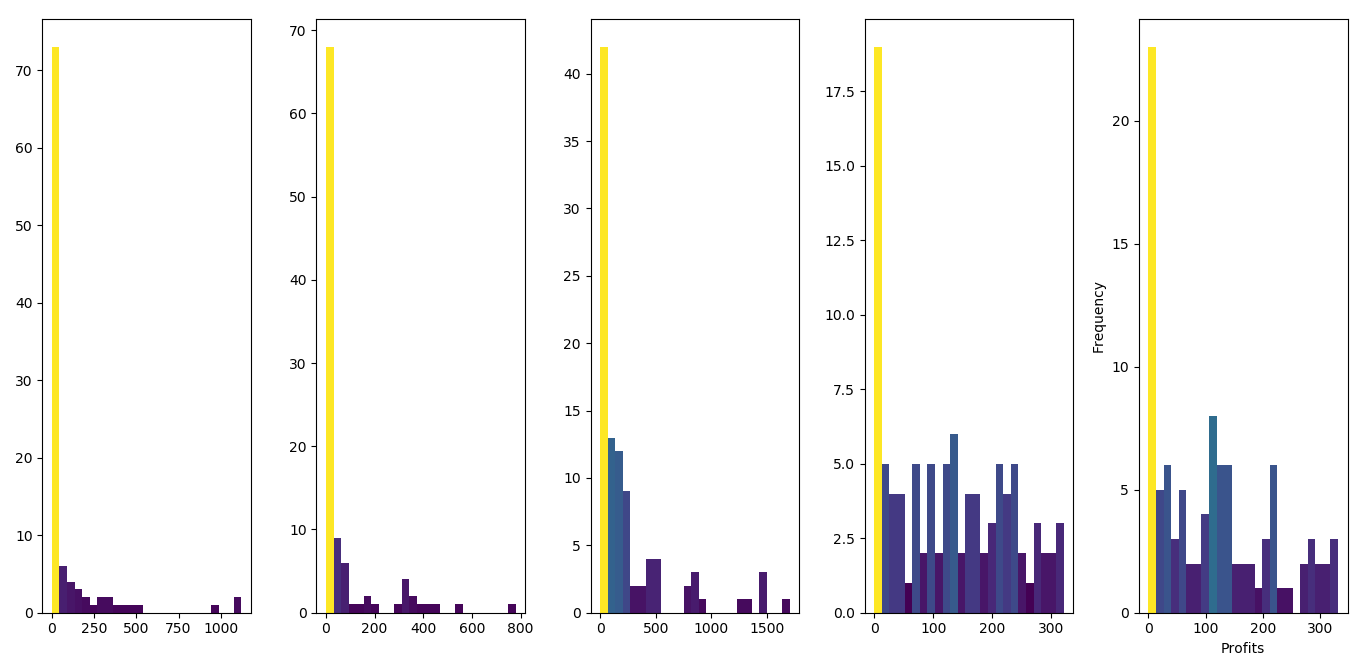
\includegraphics[width=1.0\textwidth]{fig_hist_profits5_t}
  \caption{Distribution of Consumer Surplus}
  \centering
    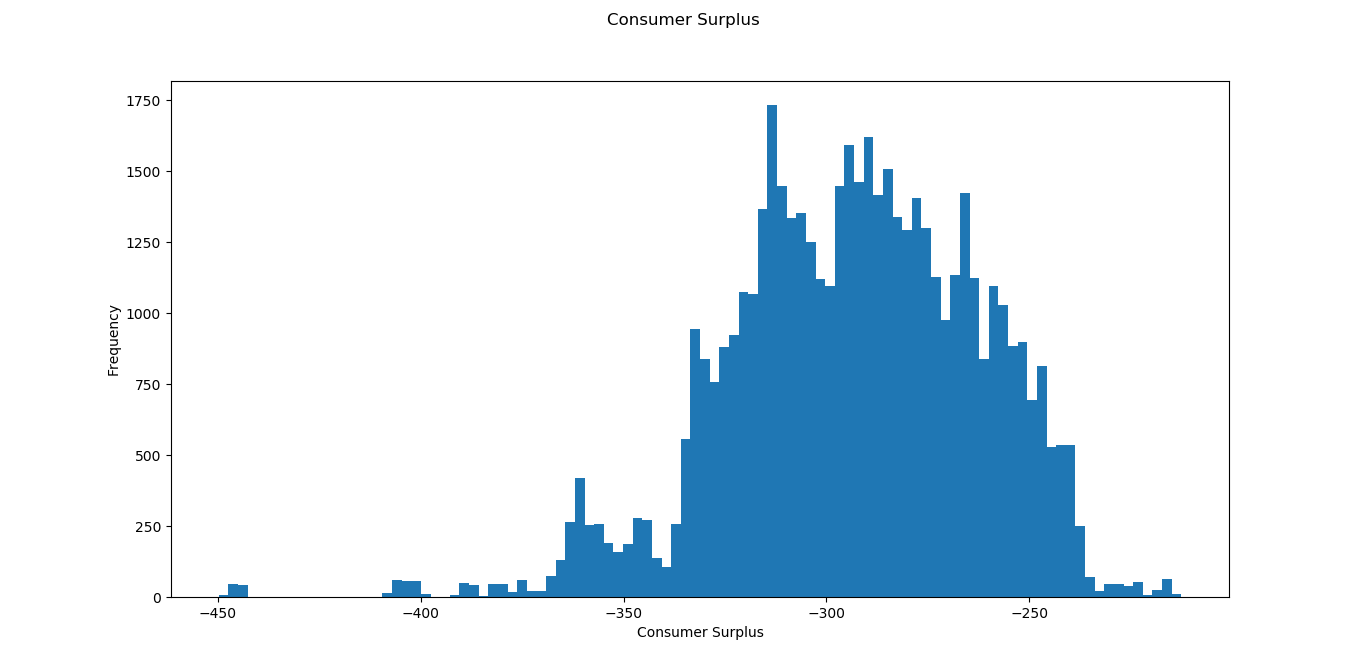
\includegraphics[width=1.0\textwidth]{fig_hist_consumersurplus5_t}
\end{figure}
\FloatBarrier

\newpage
\section{Section II}

In answering questions from this section, I assumed that $J=3$ and $M=100$, except in the case of comparison to $M=10$.

\subsection{Question 1}

\subsubsection{(a) Computation of Moments}

The value of computed moments are listed below, given assumptions $E(\xi|X)=0$ and $E(\xi|p)=0$.
$$E(\xi_{jm}X_{jm})=0.09973446265023281$$
$$E(\xi_{jm}p_{jm})=44.46994756$$
$$E(\xi_{jm}\bar{p}_{jm})=0.33463495$$

\subsubsection{(b) Validity of Moments}

The valid moments in this instance would be $E(\xi_{jm}X_{jm})$ and possibly $E(\xi_{jm}\bar{p}_{jm})$ given their proximity to 0. $E(\xi_{jm}p_{jm})$ would not be valid given price endogeneity, necessitating instrument variable approach.

\subsubsection{(c) Use of BLP and Nevo Instruments}

Given observed sample moments it would be possible to use both BLP and Nevo instruments in the instrument variables approach.

\subsection{Question 2}

\subsubsection{(a) Computation of Moments}

The BLP moment is as follows.

$$X_1=(X', P')$$
$$\theta_1=(\beta, \alpha)$$
$$E(\xi_{jm} Z)=( \delta - X_1 \theta_1 )'Z=0$$

\subsubsection{(b) Construction of Objective Function}

Given that my instrument variables are denoted by $Z$ and weighting matrix of $A$, and my parameters are specified as $\theta_1=\{ \beta, \alpha \}$ and $\theta_2=\{ \sigma_\alpha \}$, I used a contraction mapping procedure to estimate mean utility $\delta$ over numerous iterations given a tolerance until convergence. My instrument variable $Z$ is constructed with the inclusion of $X$ and non-self product characteristics.

\par Using this estimated mean utility, I constructed my objective function and minimised over $\theta_2$ only by non-linear search, while re-estimating $\theta_1$ using a first order condition within the loop. $X$ is a vector including characteristics and prices across all markets. My initial guess for $\delta_0$ were the given market shares, which were used to obtain initial starting values for parameters $\theta_1$ for subsequent iterations.

$$A=Z'Z$$
$$\omega (\theta_1) = \delta - X_1 \theta_1$$
$$\hat{\theta_1}=(X_1'Z(A)^{-1}Z'X_1)^{-1}(X_1'Z(A)^{-1}Z'\delta (\hat{\theta_2}))$$
$$\hat{\theta_2}=\underset{\theta}{argmin}\:(\omega (\hat{\theta_1})'Z) (A)^{-1} (Z'\omega (\hat{\theta_1})) $$

\subsubsection{(c) Estimation of $\theta$ Parameters}

An error with my prediction of market shares function has led to the generation of poor estimates for $\theta_1$ given prior knowledge of the true distribution of each variable.

$$\hat{\beta_0}=25.36425337\:(0.1156)$$
$$\hat{\beta_1}=-1.48315299\:(3.0040)$$
$$\hat{\beta_2}=0.18493143\:(0.0401)$$
$$\hat{\alpha}=-8.37344604\:(0.0036)$$
$$\hat{\sigma_{\alpha}}=1.075\:(1.2652)$$

We observe statistical insignificance in all estimators with the exception of $\hat{\beta_2}$ and $\hat{\alpha}$. Code output reporting variances are as follows.

% Code Snippet
\begin{lstlisting}
Estimation of Parameters and respective Standard Errors:
Beta[0]:     [25.36425337]; (0.11561192456479381) 0.013366117101575576
Beta[1]:     [-1.48315299]; (3.004018606720816) 9.024127789524872
Beta[2]:     [0.18493143]; (0.04011846630681128) 0.001609491338810752
Alpha:       [-8.37344604]; (0.003586413934865264) 1.2862364912195745e-05
Sigma Alpha: [1.075]; (1.265210529517815) 1.6007576840027502
\end{lstlisting}

\subsubsection{(d) Estimated Distributions}

The distribution of profits do not change greatly for each product from generating the same figures from the dataset using the true parameters. The distribution of the Consumer Surplus is smoother given our estimated parameters with a slightly flattened peak around the centred mean.

\begin{figure}[h]
  \caption{Distribution of Profits}
  \centering
    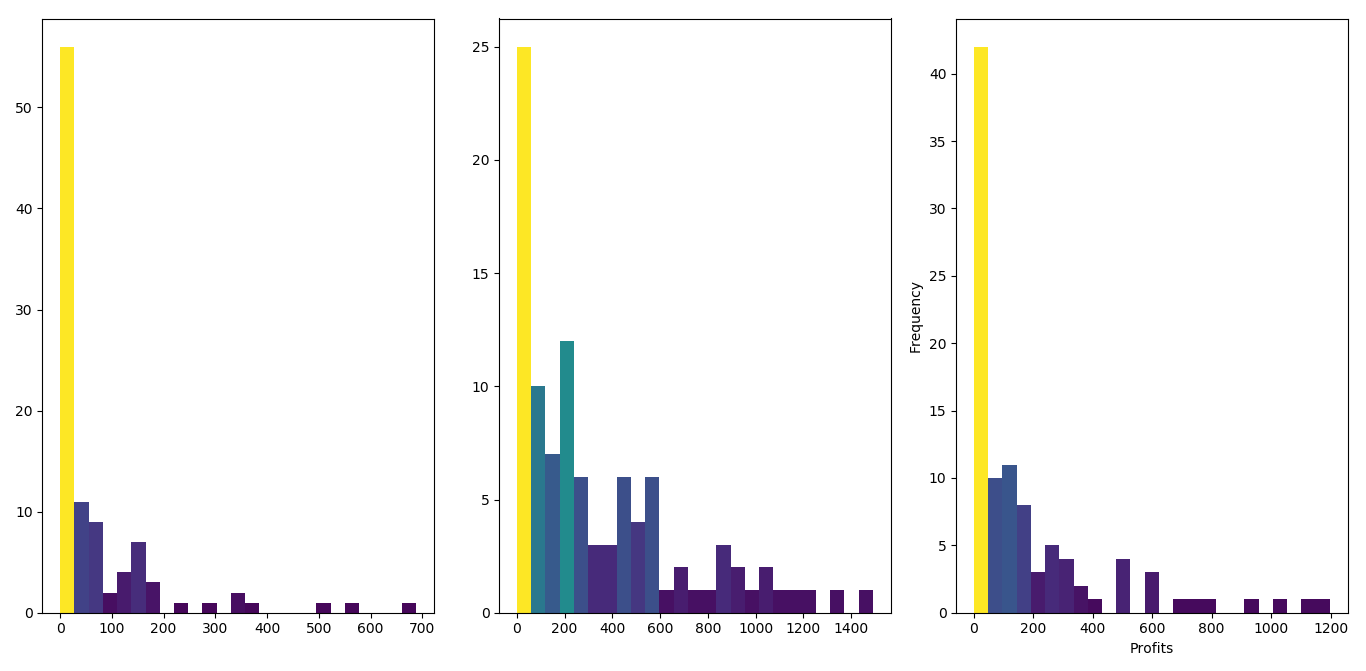
\includegraphics[width=1.0\textwidth]{fig_hist_profits3_e}
  \caption{Distribution of Consumer Surplus}
  \centering
    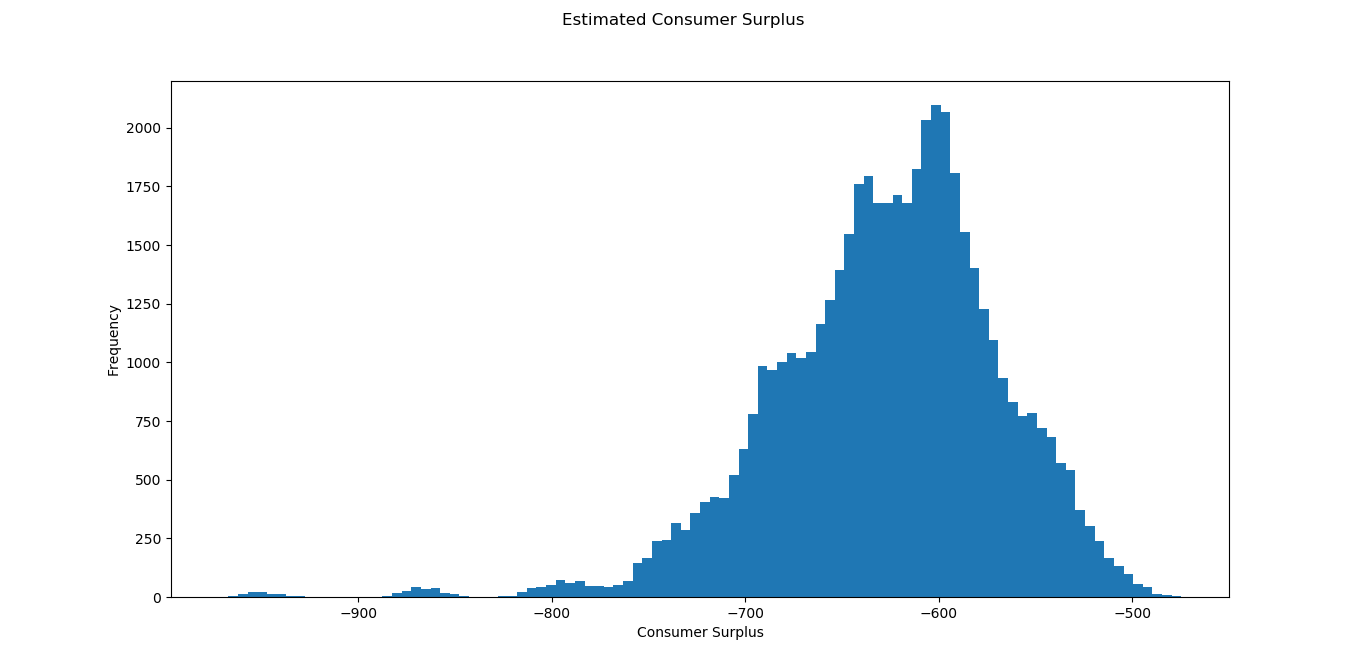
\includegraphics[width=1.0\textwidth]{fig_hist_consumersurplus3_e}
\end{figure}
\FloatBarrier

\subsubsection{(e) Estimation with Small Market Size}

The following assumes that $J=3$ and $M=10$. Estimated parameters are as follows.

$$\hat{\beta_0}=4.93649959\:(0.5500)$$
$$\hat{\beta_1}=-6.26911567\:(3.6350)$$
$$\hat{\beta_2}=0.64225405\:(2.7504)$$
$$\hat{\alpha}=-3.05454773\:(0.0680)$$
$$\hat{\sigma_{\alpha}}=1.05\:(1.6873)$$

We observe statistical insignificance in all estimators. Unusually, estimates come closer to true parameter values given the smaller market size. This is again due to aforementioned inadequacies in the share prediction function with which the contraction mapping is iterated to determine mean utility. Predictably, given large sample asymptotics, standard errors for each parameter grow higher as the size of the sample is smaller, implying a lack of precision. Code output reporting variances are as follows.

% Code Snippet
\begin{lstlisting}
Estimation of Parameters and respective Standard Errors:
Beta[0]:     [4.93649959]; (0.5500157661303665) 0.302517342991974
Beta[1]:     [-6.26911567]; (3.634987444230612) 13.213133719714198
Beta[2]:     [0.64225405]; (2.7504394588441516) 7.5649172167669105
Alpha:       [-3.05454773]; (0.06798615060671363) 0.004622116674318748
Sigma Alpha: [1.05]; (1.6872506698774878) 2.846814823002031
\end{lstlisting}

\begin{figure}[h]
  \caption{Distribution of Profits}
  \centering
    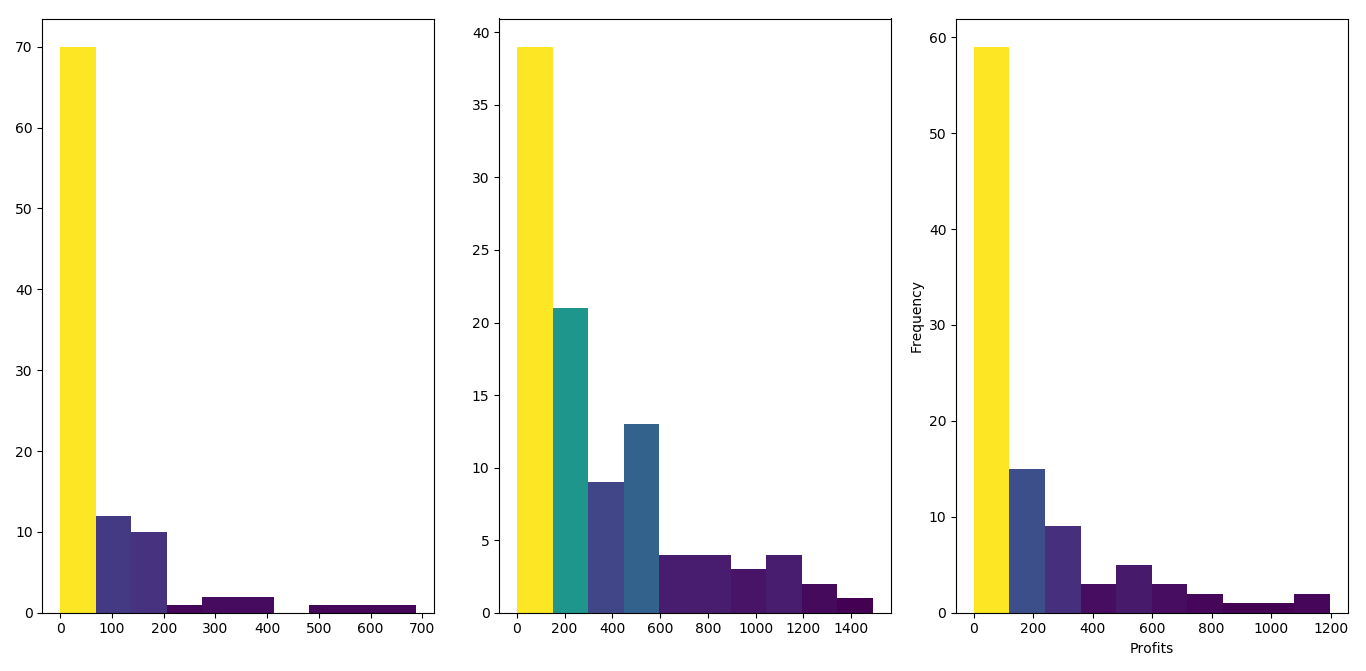
\includegraphics[width=1.0\textwidth]{fig_hist_profits10_e}
  \caption{Distribution of Consumer Surplus}
  \centering
    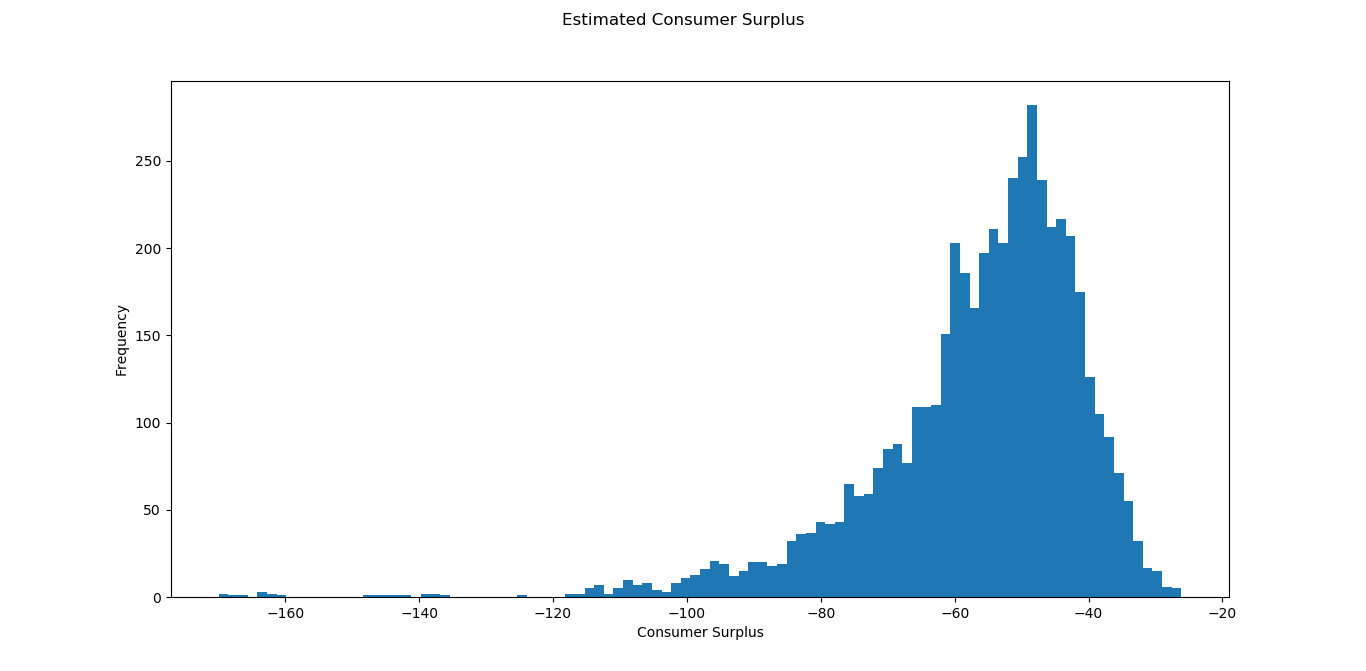
\includegraphics[width=1.0\textwidth]{fig_hist_consumersurplus10_e}
\end{figure}
\FloatBarrier

\newpage
\newpage
\section{Section III}
\subsection{Question 1}

\subsubsection{(a) Computation of Moments}
$$X_1=(X', P')$$
$$\theta_1=(\beta, \alpha)$$
$$Z=(X', W')$$
$$E(\xi_{jm} Z)=( \delta - X_1 \theta_1 )'Z=0$$

\subsubsection{(b) Estimation of $\theta$ Parameters}
Given that my instrument variables are denoted by $Z$ and weighting matrix of $A$, and my parameters are specified as $\theta_1=\{ \beta, \alpha \}$ and $\theta_2=\{ \sigma_\alpha \}$, I used a contraction mapping procedure to estimate mean utility $\delta$ over numerous iterations given a tolerance until convergence. The key difference here is that my instrument variable $Z$ is constructed with the inclusion of $X$, $W$ (supply side), and non-self product characteristics.

\par Using this estimated mean utility, I constructed my objective function and minimised over $\theta_2$ only by non-linear search, while re-estimating $\theta_1$ using a first order condition within the loop. $X$ is a vector including characteristics and prices across all markets. My initial guess for $\delta_0$ were the given market shares, which were used to obtain initial starting values for parameters $\theta_1$ for subsequent iterations.

$$\hat{\beta_0}=3.44581615\:(1.7764)$$
$$\hat{\beta_1}=-0.26703854\:(2.1939)$$
$$\hat{\beta_2}=-0.07335316\:(0.0440)$$
$$\hat{\alpha}=-1.47744888\:(0.0819)$$
$$\hat{\sigma_{\alpha}}=-0.025\:(0.9368)$$

We observe statistical insignificance in all estimators with the exception of $\hat{\beta_2}$.

% Code Snippet
\begin{lstlisting}
Estimation of Parameters and respective Standard Errors:
Beta[0]:     [3.44581615]; (1.7763856722429023) 3.155546056549868
Beta[1]:     [-0.26703854]; (2.1939101073905936) 4.8132415593106055
Beta[2]:     [-0.07335316]; (0.044034215343053545) 0.0019390121208784123
Alpha:       [-1.47744888]; (0.08189215439712716) 0.006706324951802914
Sigma Alpha: [-0.025]; (0.936762973259827) 0.8775248680705915
\end{lstlisting}

\begin{figure}[h]
  \caption{Distribution of Profits}
  \centering
    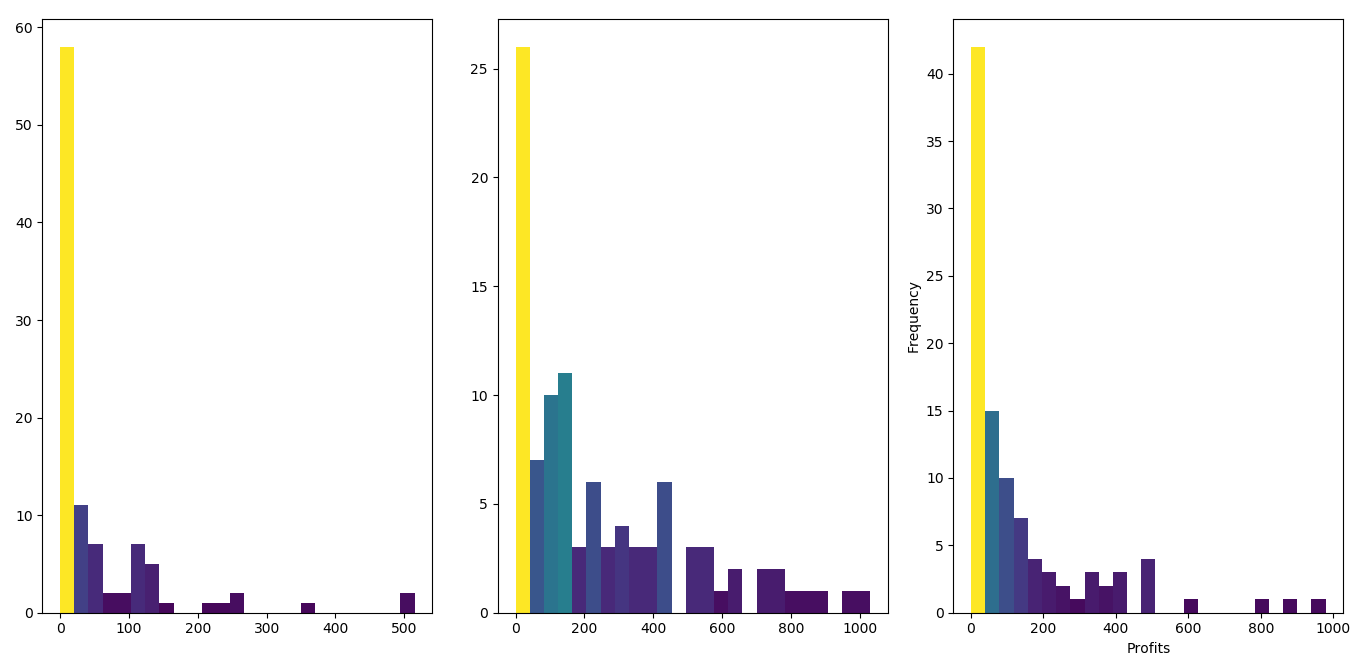
\includegraphics[width=1.0\textwidth]{fig_hist_profitsW3_e}
  \caption{Distribution of Consumer Surplus}
  \centering
    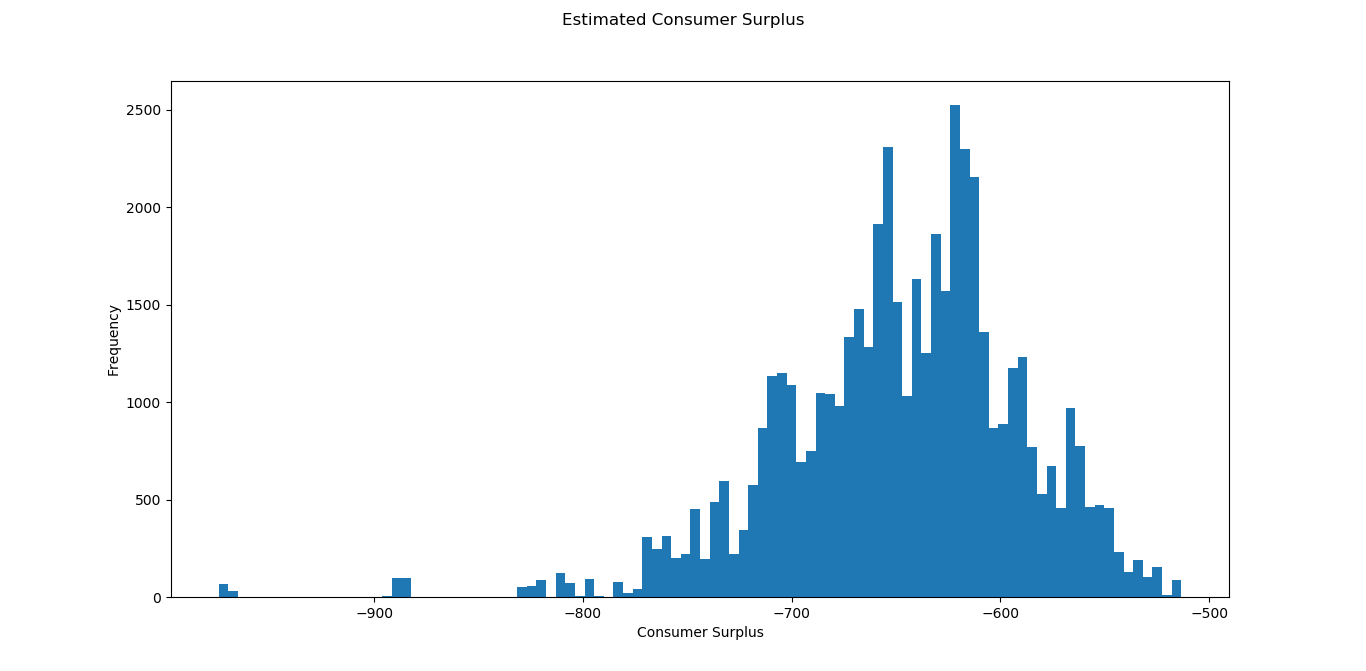
\includegraphics[width=1.0\textwidth]{fig_hist_consumersurplusW3_e}
\end{figure}
\FloatBarrier

\subsubsection{(c) Estimation with Small Market Size}

The following assumes that $J=3$ and $M=10$. Estimated parameters are as follows.

$$\hat{\beta_0}=7.200781\:(1.4963)$$
$$\hat{\beta_1}=-3.14960642\:(14.1955)$$
$$\hat{\beta_2}=0.67499153\:(5.8012)$$
$$\hat{\alpha}=-4.10794263\:(0.0266)$$
$$\hat{\sigma_{\alpha}}=1.\:(6.6877)$$

Expectedly, estimates stray farther than true parameter values and also in comparison to prior estimation, given the smaller market size. This is again due to aforementioned inadequacies in the share prediction function with which the contraction mapping is iterated to determine mean utility. Predictably, given large sample asymptotics, standard errors for each parameter grow higher as the size of the sample is smaller, implying a lack of precision.

\par Statistical insignificance persists overall, however $\hat{\alpha}$ appears to be statistically significant in this estimation compared to the case with 100 markets. Distributions follow closely, however, Consumer Surplus is considerably smoother without twin peaks in the case of the smaller market. Code output reporting variances are as follows.

% Code Snippet
\begin{lstlisting}
Estimation of Parameters and respective Standard Errors:
Beta[0]:     [7.200781]; (1.4962813893043092) 2.238857995978434
Beta[1]:     [-3.14960642]; (14.195538337691184) 201.51330869686018
Beta[2]:     [0.67499153]; (5.8012724739414185) 33.654762316910386
Alpha:       [-4.10794263]; (0.026634193525163823) 0.0007093802647358785
Sigma Alpha: [1.]; (6.687712926310157) 44.72550418473597
\end{lstlisting}

\begin{figure}[h]
  \caption{Distribution of Profits}
  \centering
    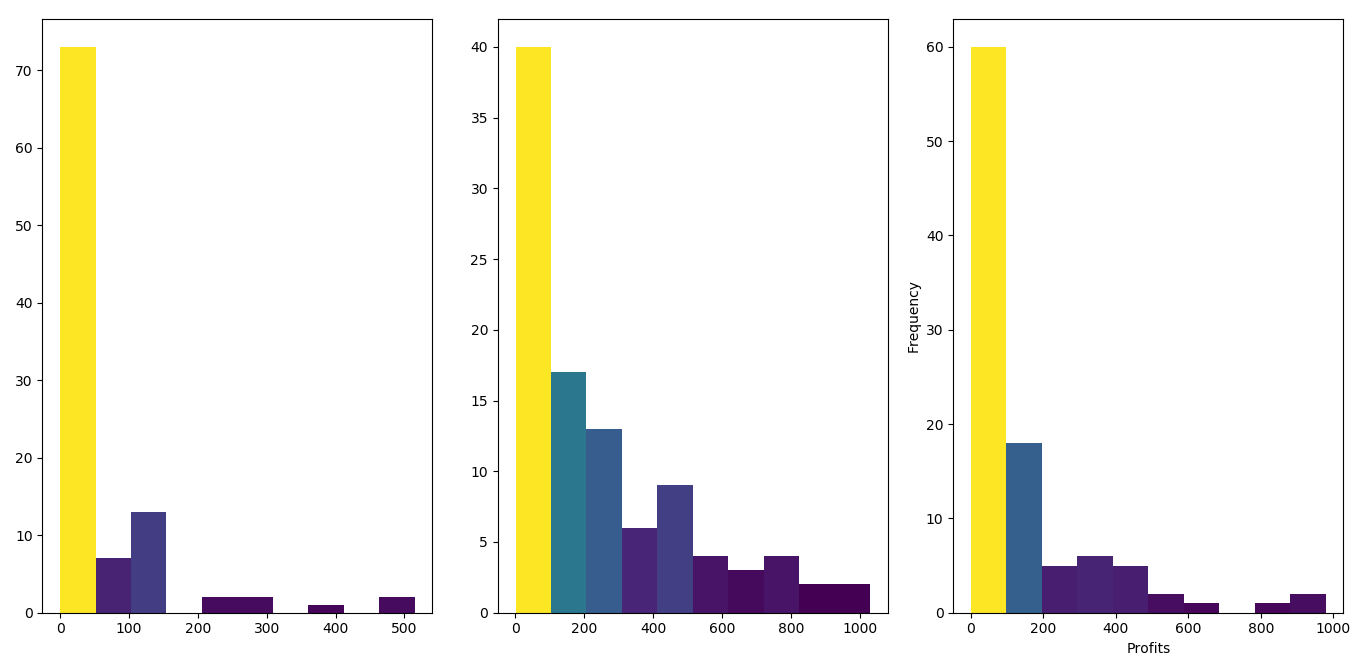
\includegraphics[width=1.0\textwidth]{fig_hist_profitsW10_e}
  \caption{Distribution of Consumer Surplus}
  \centering
    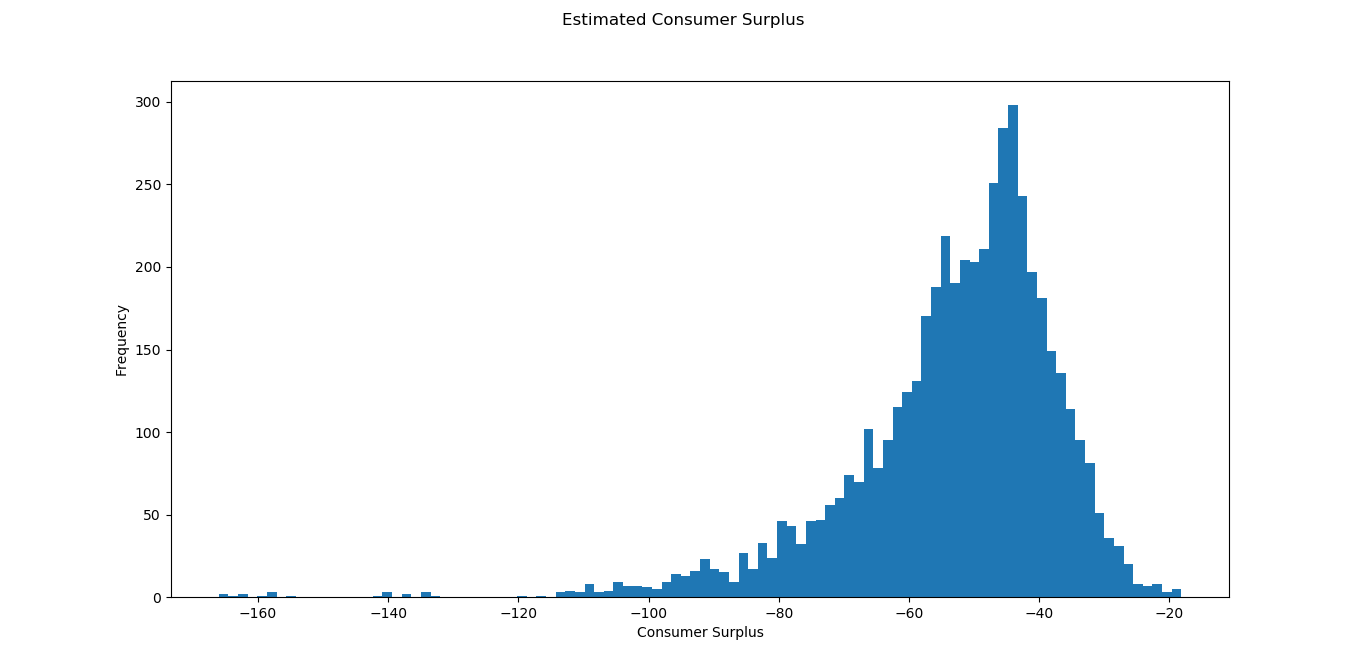
\includegraphics[width=1.0\textwidth]{fig_hist_consumersurplusW10_e}
\end{figure}
\FloatBarrier

\newpage
\section{Appendix: Source Code}
\subsection{Source}

\lstinputlisting[language=Python]{pset1_SMSajidAlSanai.py}

\end{document}